\subsubsection{Overview}

The SmartRobotinoInstructionPlanner component is currently responsible of the task coordinantion between all components of the Robocup Logistics Software. The intention of the previous team was that a master robot should process the information from the Robocup Logistics Refereebox and start instruction all other robots. The scenario application like driving, docking or detection should be implemented in the SmartLispServer component using the SmartTCL language. \\

The SmartRobotinoInstructionPlanner is connected to the Refbox Component using a bi-directional SmartSoft port. For transmitting data between those two components various communication objects are used. To the other components like the SmartMPSDetection, SmartAlvarTagDetection or the components which provide services like mapping or driving, the SmartRobotinoInstructionPlanner uses SmartTCL messages which are transferred by using strings and communication ports. 


\subsubsection{Previous implementation}

As described in (reference to book of knowledge) the InstructionPlanner was designed for planning and coordination of other components on the master robotino (the one who manages the connection between the Refbox and all robotinos) but also all other robotinos. This means that it was designed that on all slave robotinos only the necessary parts like driving, detection or docking should run. All coordination should be done by the instruction planner on the master robotino. The intention behind this idea was that the referee box was sending a list of probable zone which can contain a MPS station for detection. This list of MPS stations was then splitted by an algorithm into three parts (one for each robot), so that a concurrent exploration and detection of the gamefield can be archieved. In the 2017 scenario (link to 2017 rules) this feature was discarded from the competition. In the newer scenario there is no information whether there is a MPS station or not. Therefore this feature was also discared in the new design for the 2017 competition \ref{sec:new_design}.  \\



\subsubsection{New Design}
\label{sec:new_design}
Describe the overall design of the instruction planner. Which ports are used and connected to other components. What are the tasks of the component and what purpose do they fulfill. 

\begin{figure}[h]
\centering
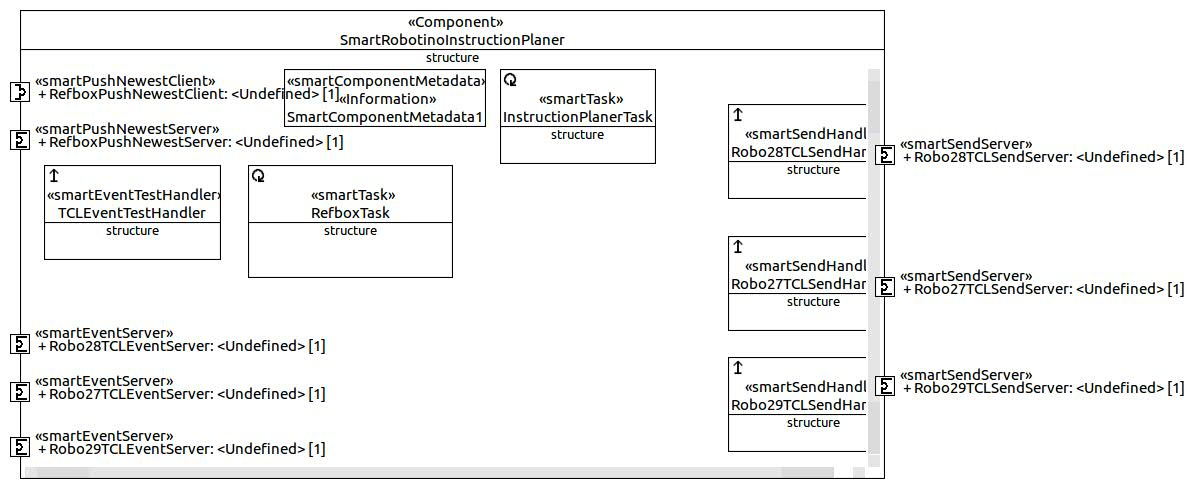
\includegraphics[scale=0.25]{pic/SmartRobotinoInstructionPlaner.JPG}
\caption{Model of InstructionPlanner}
\end{figure}


\subsubsection{Communication Objects}

Describe the messages which are processed by the instruction planner. 

\begin{itemize}

\item CommRefbox \\

Describes the messages which come from the Refbox. This means that in this CommunicationObjecs the 
Phases and States of the running tournament are encoded.

\item MachineInfo \\

The MachineInfo communication object is used to handover the information of detected MPS stations to the SmartRefBoxServer component. 

\item MachineReport \\

\item RobotInfo \\

The RobotInfo is used to send the current state of the robot from the point of the refbox. This message is send from SmartRefboxServer to InstructionPlanner. 

\end{itemize}


\subsubsection{Statemachine}

Describe the state machine with a diagram with states
and transitions

\subsubsection{Maintenance Modes}

Describe how to team and the robot can react to failures and the system. How to set the robot into maintenance mode and how the robot can return to the game. 


\subsubsection{Outcome}

Multiple robots and Production phase







